\documentclass[11pt,preprint, authoryear]{elsarticle}

\usepackage{lmodern}
%%%% My spacing
\usepackage{setspace}
\setstretch{1.2}
\DeclareMathSizes{12}{14}{10}{10}

% Wrap around which gives all figures included the [H] command, or places it "here". This can be tedious to code in Rmarkdown.
\usepackage{float}
\let\origfigure\figure
\let\endorigfigure\endfigure
\renewenvironment{figure}[1][2] {
    \expandafter\origfigure\expandafter[H]
} {
    \endorigfigure
}

\let\origtable\table
\let\endorigtable\endtable
\renewenvironment{table}[1][2] {
    \expandafter\origtable\expandafter[H]
} {
    \endorigtable
}


\usepackage{ifxetex,ifluatex}
\usepackage{fixltx2e} % provides \textsubscript
\ifnum 0\ifxetex 1\fi\ifluatex 1\fi=0 % if pdftex
  \usepackage[T1]{fontenc}
  \usepackage[utf8]{inputenc}
\else % if luatex or xelatex
  \ifxetex
    \usepackage{mathspec}
    \usepackage{xltxtra,xunicode}
  \else
    \usepackage{fontspec}
  \fi
  \defaultfontfeatures{Mapping=tex-text,Scale=MatchLowercase}
  \newcommand{\euro}{€}
\fi

\usepackage{amssymb, amsmath, amsthm, amsfonts}

\def\bibsection{\section*{References}} %%% Make "References" appear before bibliography


\usepackage[round]{natbib}

\usepackage{longtable}
\usepackage[margin=2.3cm,bottom=2cm,top=2.5cm, includefoot]{geometry}
\usepackage{fancyhdr}
\usepackage[bottom, hang, flushmargin]{footmisc}
\usepackage{graphicx}
\numberwithin{equation}{section}
\numberwithin{figure}{section}
\numberwithin{table}{section}
\setlength{\parindent}{0cm}
\setlength{\parskip}{1.3ex plus 0.5ex minus 0.3ex}
\usepackage{textcomp}
\renewcommand{\headrulewidth}{0pt}

\usepackage{array}
\newcolumntype{x}[1]{>{\centering\arraybackslash\hspace{0pt}}p{#1}}

%%%%  Remove the "preprint submitted to" part. Don't worry about this either, it just looks better without it:
\makeatletter
\def\ps@pprintTitle{%
  \let\@oddhead\@empty
  \let\@evenhead\@empty
  \let\@oddfoot\@empty
  \let\@evenfoot\@oddfoot
}
\makeatother

 \def\tightlist{} % This allows for subbullets!

\usepackage{hyperref}
\hypersetup{breaklinks=true,
            bookmarks=true,
            colorlinks=true,
            citecolor=blue,
            urlcolor=blue,
            linkcolor=blue,
            pdfborder={0 0 0}}


% The following packages allow huxtable to work:
\usepackage{siunitx}
\usepackage{multirow}
\usepackage{hhline}
\usepackage{calc}
\usepackage{tabularx}
\usepackage{booktabs}
\usepackage{caption}


\newenvironment{columns}[1][]{}{}

\newenvironment{column}[1]{\begin{minipage}{#1}\ignorespaces}{%
\end{minipage}
\ifhmode\unskip\fi
\aftergroup\useignorespacesandallpars}

\def\useignorespacesandallpars#1\ignorespaces\fi{%
#1\fi\ignorespacesandallpars}

\makeatletter
\def\ignorespacesandallpars{%
  \@ifnextchar\par
    {\expandafter\ignorespacesandallpars\@gobble}%
    {}%
}
\makeatother

\newlength{\cslhangindent}
\setlength{\cslhangindent}{1.5em}
\newenvironment{CSLReferences}%
  {\setlength{\parindent}{0pt}%
  \everypar{\setlength{\hangindent}{\cslhangindent}}\ignorespaces}%
  {\par}


\urlstyle{same}  % don't use monospace font for urls
\setlength{\parindent}{0pt}
\setlength{\parskip}{6pt plus 2pt minus 1pt}
\setlength{\emergencystretch}{3em}  % prevent overfull lines
\setcounter{secnumdepth}{5}

%%% Use protect on footnotes to avoid problems with footnotes in titles
\let\rmarkdownfootnote\footnote%
\def\footnote{\protect\rmarkdownfootnote}
\IfFileExists{upquote.sty}{\usepackage{upquote}}{}

%%% Include extra packages specified by user
\usepackage{booktabs}
\usepackage{longtable}
\usepackage{array}
\usepackage{multirow}
\usepackage{wrapfig}
\usepackage{float}
\usepackage{colortbl}
\usepackage{pdflscape}
\usepackage{tabu}
\usepackage{threeparttable}
\usepackage{threeparttablex}
\usepackage[normalem]{ulem}
\usepackage{makecell}
\usepackage{xcolor}

%%% Hard setting column skips for reports - this ensures greater consistency and control over the length settings in the document.
%% page layout
%% paragraphs
\setlength{\baselineskip}{12pt plus 0pt minus 0pt}
\setlength{\parskip}{12pt plus 0pt minus 0pt}
\setlength{\parindent}{0pt plus 0pt minus 0pt}
%% floats
\setlength{\floatsep}{12pt plus 0 pt minus 0pt}
\setlength{\textfloatsep}{20pt plus 0pt minus 0pt}
\setlength{\intextsep}{14pt plus 0pt minus 0pt}
\setlength{\dbltextfloatsep}{20pt plus 0pt minus 0pt}
\setlength{\dblfloatsep}{14pt plus 0pt minus 0pt}
%% maths
\setlength{\abovedisplayskip}{12pt plus 0pt minus 0pt}
\setlength{\belowdisplayskip}{12pt plus 0pt minus 0pt}
%% lists
\setlength{\topsep}{10pt plus 0pt minus 0pt}
\setlength{\partopsep}{3pt plus 0pt minus 0pt}
\setlength{\itemsep}{5pt plus 0pt minus 0pt}
\setlength{\labelsep}{8mm plus 0mm minus 0mm}
\setlength{\parsep}{\the\parskip}
\setlength{\listparindent}{\the\parindent}
%% verbatim
\setlength{\fboxsep}{5pt plus 0pt minus 0pt}



\begin{document}



\begin{frontmatter}  %

\title{Analysis of ZAR Volatility and Performance}

% Set to FALSE if wanting to remove title (for submission)




\author[Add1]{Jonathan Rossouw}
\ead{20858345@sun.ac.za}







\begin{abstract}
\small{
This document provides an analysis of the recent ZAR performance. The
ZAR has been among the most volatile currencies in the recent past. Here
the smoothed volatility is modelled using the GARCH method. The smoothed
volatility is compared to global volatility. The performance of the ZAR
is also determined for different periods.
}
\end{abstract}

\vspace{1cm}





\vspace{0.5cm}

\end{frontmatter}



%________________________
% Header and Footers
%%%%%%%%%%%%%%%%%%%%%%%%%%%%%%%%%
\pagestyle{fancy}
\chead{}
\rhead{}
\lfoot{}
\rfoot{}
\lhead{}
%\rfoot{\footnotesize Page \thepage } % "e.g. Page 2"
\cfoot{}

%\setlength\headheight{30pt}
%%%%%%%%%%%%%%%%%%%%%%%%%%%%%%%%%
%________________________

\headsep 35pt % So that header does not go over title




\hypertarget{introduction}{%
\section{\texorpdfstring{Introduction
\label{Introduction}}{Introduction }}\label{introduction}}

The ZAR has been among the most volatile currencies in the recent past.
Here the smoothed volatility is modelled using the GARCH method. The
smoothed volatility is compared to global volatility. The performance of
the ZAR is also determined for different periods.

\hypertarget{garch-model}{%
\section{GARCH Model}\label{garch-model}}

From the Return Type Persistence plot, it is clear that there is a level
of conditional heteroskedasticity. This is clear from the region of
large squared returns. The ACF's of the dlog returns show limited
autocorrelation in returns, but the ACF's of squared and absolute
returns indicate autocorrelation. This coupled with the Box-Ljung test
rejecting the hypothesis of no autocorrelation in teh squared returns
indicates the need for a GARCH type model.

\par

The type of GARCH model that results in the lowest AIC is the gjrGARCH
specification. This allows for leverage effects. The fitted gjrGARCH
model gives the output as seen in Table \ref{tab:coef}. The plot
comparing the squared returns to the GARCH smoothed returns shows the
model smoothes out the noise from the signal.

\begin{verbatim}
## $`Return Plots`
\end{verbatim}

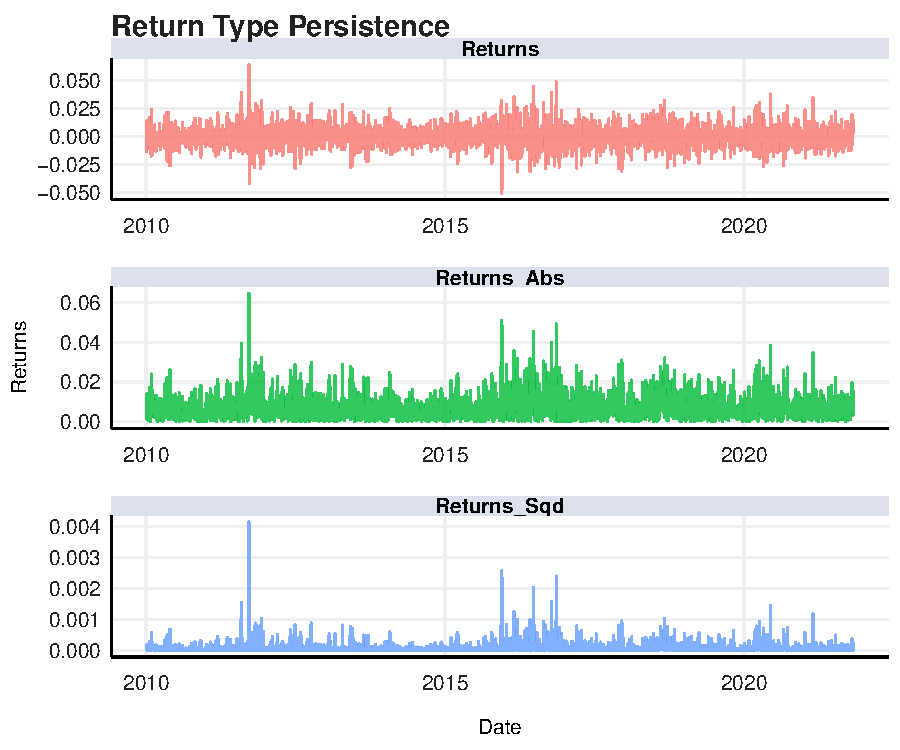
\includegraphics{Question4_files/figure-latex/q4_2-1.pdf}

\begin{verbatim}
## 
## $`ACF Plots`
\end{verbatim}

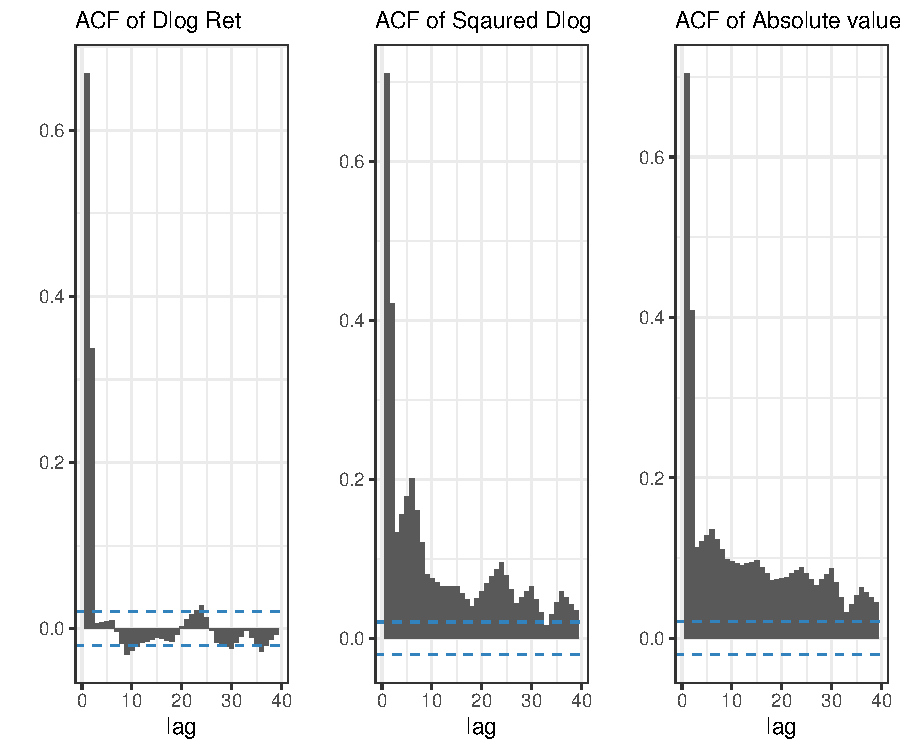
\includegraphics{Question4_files/figure-latex/q4_2-2.pdf}

\begin{verbatim}
## 
## $`Box Statistics`
## 
##  Box-Ljung test
## 
## data:  data$dlogret^2
## X-squared = 303.93, df = 12, p-value < 2.2e-16
\end{verbatim}

\begin{verbatim}
##                 sGARCH  gjrGARCH    eGARCH    apARCH
## Akaike       -6.510600 -6.519711 -6.517530 -6.515322
## Bayes        -6.500820 -6.507975 -6.505794 -6.501630
## Shibata      -6.510605 -6.519718 -6.517537 -6.515332
## Hannan-Quinn -6.507087 -6.515495 -6.513314 -6.510404
\end{verbatim}

\begin{table}

\caption{\label{tab:coef}GARCH Coefficients}
\centering
\begin{tabular}[t]{l|r|r|r|r}
\hline
  &  Estimate &  Std. Error &  t value & Pr(>|t|)\\
\hline
mu & 0.000 & 0.000 & 1.356 & 0.175\\
\hline
ar1 & -0.007 & 0.018 & -0.379 & 0.705\\
\hline
omega & 0.000 & 0.000 & 1.688 & 0.091\\
\hline
alpha1 & 0.060 & 0.008 & 7.764 & 0.000\\
\hline
beta1 & 0.954 & 0.005 & 176.375 & 0.000\\
\hline
gamma1 & -0.057 & 0.010 & -5.538 & 0.000\\
\hline
shape & 12.959 & 2.759 & 4.697 & 0.000\\
\hline
\end{tabular}
\end{table}

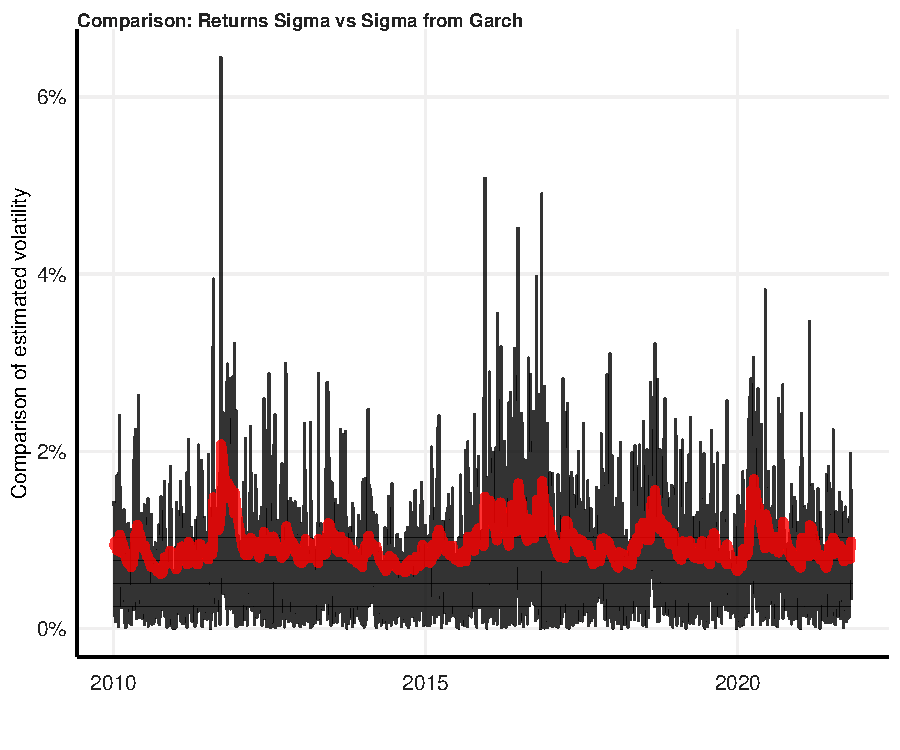
\includegraphics{Question4_files/figure-latex/q4_2-3.pdf}

\hypertarget{zar-vol}{%
\section{ZAR Vol}\label{zar-vol}}

From Table \ref{tab:vol}, it is clear that the ZAR has been the fourth
most volatile currency over the past decade.

\begin{table}

\caption{\label{tab:vol}Top 10 Highest Mean Squared Returns}
\centering
\begin{tabular}[t]{l|r}
\hline
Name & Mean\_Vol\\
\hline
Ghana\_Cncy & 0.0001712\\
\hline
Russia\_Cncy & 0.0001006\\
\hline
Brazil\_Cncy & 0.0000968\\
\hline
SouthAfrica\_Cncy & 0.0000939\\
\hline
Zambia\_Cncy & 0.0000893\\
\hline
Argentina\_Cncy & 0.0000877\\
\hline
Nigeria\_Cncy & 0.0000863\\
\hline
Turkey\_Cncy & 0.0000801\\
\hline
Egypt\_Cncy & 0.0000765\\
\hline
Hungary\_Cncy & 0.0000644\\
\hline
\end{tabular}
\end{table}

\hypertarget{zar-vol-and-global-vol}{%
\section{ZAR Vol and Global Vol}\label{zar-vol-and-global-vol}}

The below figure compares the smoothed volatility from the above GARCH
model for the ZAR and the mean daily currency volatility index. In the
beginning of the decade, the ZAR and global vol were not alined.
However, since 2016, the ZAR Vol and Global Vol have moved in tandem.
Thus ZAR Vol is a very clear proxy for Global Currency Vol.

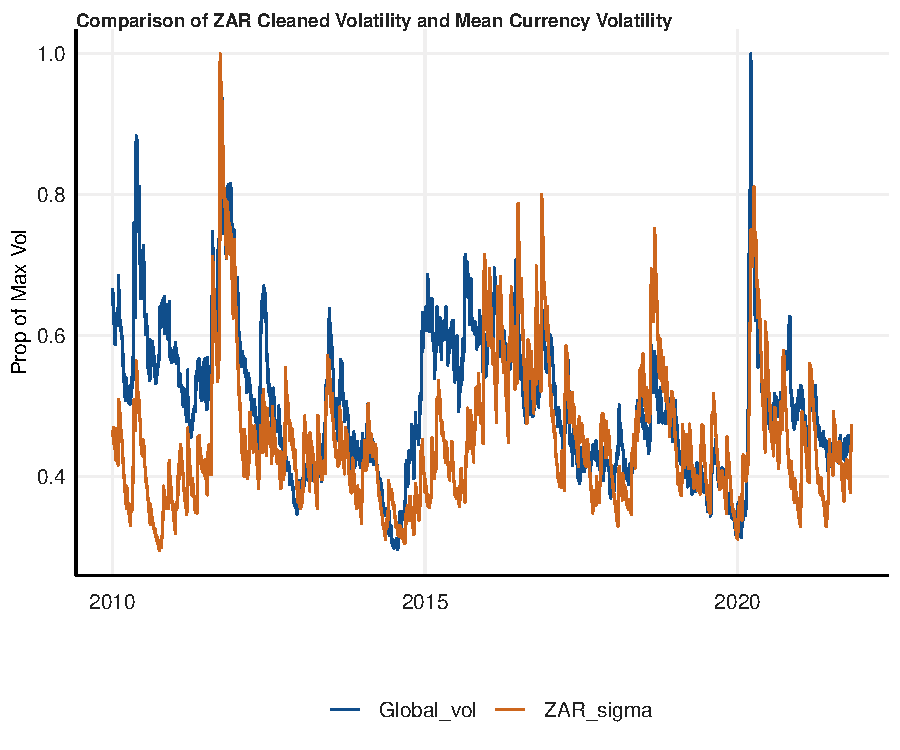
\includegraphics{Question4_files/figure-latex/q4_4-1.pdf}

\hypertarget{zar-performance}{%
\section{ZAR Performance}\label{zar-performance}}

When comparing the average performance of the ZAR during normal times
compared to periods of expected higher performance. The periods
concerned are: the top decile of carry trade returns, bottom decile of
value strategy returns, and the top decile of Dollar returns. From Table
\ref{tab:zar}, ZAR performance is higher during the selected periods
when compared to normal periods. The performance for each specified
period is the same. This indicates that the periods most likely
coincide.

\begin{table}

\caption{\label{tab:zar}ZAR Performance during Different Periods}
\centering
\begin{tabular}[t]{r|l}
\hline
Mean\_Ret & Type\\
\hline
0.0002451 & Normal\\
\hline
0.0002451 & Carry-Trade\\
\hline
0.0002451 & Value\\
\hline
0.0002451 & Basket\\
\hline
\end{tabular}
\end{table}

\bibliography{Tex/ref}





\end{document}
